
% ------------------------------------------------------------------------
\chapter{Capital expenditure}
\label{chap_capex}
The cost of a telecommunications network can be divided into capital and operational expenditures. The CAPEX is the amount of money needed to set up and install a particular network and the OPEX is the amount of money needed to run this network as well as its maintenance and operation over time \cite{capex}\cite{opex}\cite{aulas}. In this section we will only focus on CAPEX, that is the costs of installing a particular network.
The current chapter proposes and describes the optimization model used to calculate capital expenditures of the network using as a tool ILP and analytical models. These calculations are made based on the three modes of transport (opaque, transparent and translucent) with 1+1 protection and without survivability.
In the section \ref{ILP_CAPEX} it is described how the network CAPEX is calculated using ILP models and in its subsections, the calculations and constraints of the three transport modes mentioned above are identified.
In the section\ref{analytical_CAPEX} the network CAPEX is calculated using analytical models. In its subsections the calculations and constraints of the opaque and transparent modes of transport are identified.

%Section CAPEX ILP
\clearpage

\section{ILP models}\label{ILP_CAPEX}

As we know the telecommunications networks are made up of links and nodes, so it is possible to define the CAPEX as being the sum of the cost of links and cost of nodes\cite{aulas}. This can be said that the CAPEX cost in monetary units (e.g. euros, or dollars), $C_C$, is given by the equation \ref{Capex}

\begin{equation}
C_C = C_L + C_N
\label{Capex}
\end{equation}

\noindent
where $C_L$	is the link cost in monetary units (e.g. euros, or dollars) and $C_N$ is the node cost in monetary units (e.g. euros, or dollars).\\

For this calculation first let's focus on the cost of the links and for this we have to take into account the figure \ref{link_design} where we can see the design of a link. In this figure we can see that a link consists of two optical line terminals (one at each end), it also has several amplifiers (this number depends on the length of the link) placed at a certain distance (span) and finally it also consists of several optical channels each with a certain wavelength \cite{aulas}\cite{ramas2010}.\\

\begin{figure}[h!]
\centering
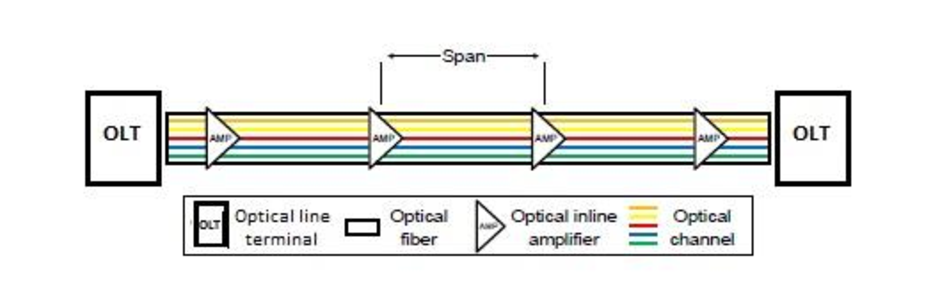
\includegraphics[width=\textwidth]{sdf/ILP/figures/link_design}
\caption{Design of a link.}
\label{link_design}
\end{figure}

\vspace{13pt}
Through the previous image, we can conclude that the link cost in monetary units (e.g. euros, or dollars), $C_L$, is calculated by the equation \ref{Capex_Link}

\begin{equation}
C_L = \sum_{i=1}^N \sum_{j=i+1}^N L_{ij} \bigg( 2 \gamma_0^{OLT} + 2 \gamma_1^{OLT} \tau W_{ij} + 2 N^R_{ij} c^R \bigg)
\label{Capex_Link}
\end{equation}

\noindent
where
\begin{itemize}
\item{$i$               $\rightarrow$   Index for start node of a physical link}
\item{$j$               $\rightarrow$   Index for end node of a physical link}
\item{$N$				$\rightarrow$	Total number of nodes, N $\in \mathbb{N}$}
\item{$L_{ij}$			$\rightarrow$	Binary variable indicating if link between the nodes $i$ and $j$ is used, $L_{ij} \in {0, 1}$}
\item{$\gamma_0^{OLT}$	$\rightarrow$	OLT cost in monetary units (e.g. euros, or dollars)}
\item{$\gamma_1^{OLT}$	$\rightarrow$	Transponder cost in monetary units (e.g. euros, or dollars)}
\item{$\tau$		    $\rightarrow$	Line bit-rate}
\item{$W_{ij}$          $\rightarrow$   Total number of optical channels in link $i$ $j$}
\item{$N^R_{ij}$    	$\rightarrow$	Number of optical amplifiers in link $i$ $j$}
\item{$c^R$				$\rightarrow$	Optical amplifiers cost in monetary units (e.g. euros, or dollars)}
\end{itemize}

\vspace{11pt}
The number of amplifiers for each link can be calculated by equation \ref{Capex_amplifiers}

\begin{equation}
N^R_{ij} = \sum_{i=1}^{N}\sum\limits_{j=i+1}^{N}\left(\left\lceil\frac{len_{ij}}{span}\right\rceil-1\right)
\label{Capex_amplifiers}
\end{equation}

\vspace{11pt}
\noindent
where the variable $len_{ij}$ is the length of link $ij$ in kilometers and the $span$ is the distance between amplifiers also in kilometers \cite{aulas}. For all cases this distance is always 100 km.\\

The next step is to take into account the cost of the nodes, but for this we must first know how a node is constituted. The nodes have an electrical part, $C_{EXC}$, and an optical part, $C_{OXC}$, so we can conclude that the cost of the nodes, $C_N$, is given by the sum of these two parts \cite{aulas} thus obtaining the equation \ref{Capex_Node}.

\begin{equation}
C_N = C_{EXC} + C_{OXC}
\label{Capex_Node}
\end{equation}

\vspace{11pt}
In relation to the electric part we can see the figure \ref{exc_design} where it shows its constitution.

\begin{figure}[h!]
\centering
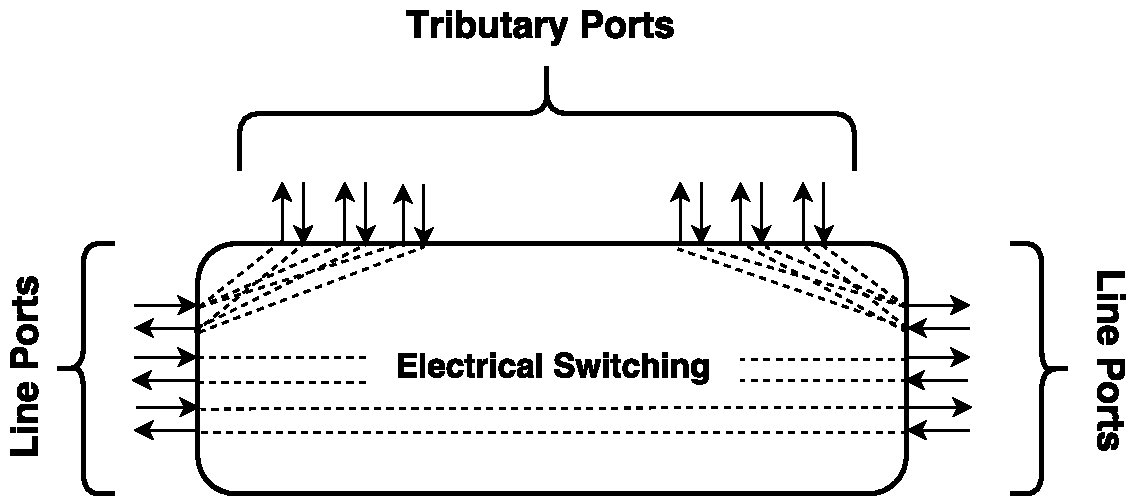
\includegraphics[width=8cm]{sdf/ILP/figures/exc_design}
\caption{Design of a electrical switching.}
\label{exc_design}
\end{figure}

Through this image, we can conclude in a simple way that the electric cost is the sum of the fixed cost of the electrical connection with the total cost of all the electric ports.\\
Therefore the electric cost in monetary units (e.g. euros, or dollars), $C_{EXC}$, is given by equation \ref{Capex_Node_EXC}\\

\begin{equation}
C_{EXC} = \sum_{n=1}^{N} N_{exc,n} \left( \gamma_{e0} + \sum_{c=-1}^B \gamma_{e1,c} P_{exc,c,n} \right)
\label{Capex_Node_EXC}
\end{equation}

\noindent
where
\begin{itemize}
\item{$N$				$\rightarrow$	Total number of nodes, N $\in \mathbb{N}$}
\item{$N_{exc,n}$		$\rightarrow$	Binary variable indicating if node $n$ is used, $N_{exc,n} \in {0, 1}$}
\item{$\gamma_{e0}$ 	$\rightarrow$	EXC cost in monetary units (e.g. euros, or dollars)}
\item{$\gamma_{e1,c}$	$\rightarrow$	EXC port cost in monetary units (e.g. euros, or dollars) with bit-rate $B$ and with a given transceiver reach}
\item{$P_{exc,c,n}$	    $\rightarrow$	Number of ports of the electrical switch}
\item{$B$           	$\rightarrow$	A natural number corresponding to the maximum index of short-reach ports, see table below}
\end{itemize}

\begin{table}[h!]
\centering
\begin{tabular}{|c|c|}
  \hline
  Index & Bit rate \\
 \hline\hline
  -1 & 100 Gbits/s line bit-rate (long-reach port) \\
  0 & 1.25 Gbits/s tributary bit-rate (short-reach port) \\
  1 & 2.5 Gbits/s tributary bit-rate (short-reach port) \\
  2 & 10 Gbits/s tributary bit-rate (short-reach port) \\
  3 & 40 Gbits/s tributary bit-rate (short-reach port) \\
  4 & 100 Gbits/s tributary bit-rate (short-reach port) \\
  \hline
\end{tabular}
\caption{Table with index and your corresponding bit rate}
\label{table_bitrate}
\end{table}

Now, in relation to the optical part through the figure \ref{oxc_design} we can see its constitution.\\

\begin{figure}[h!]
\centering
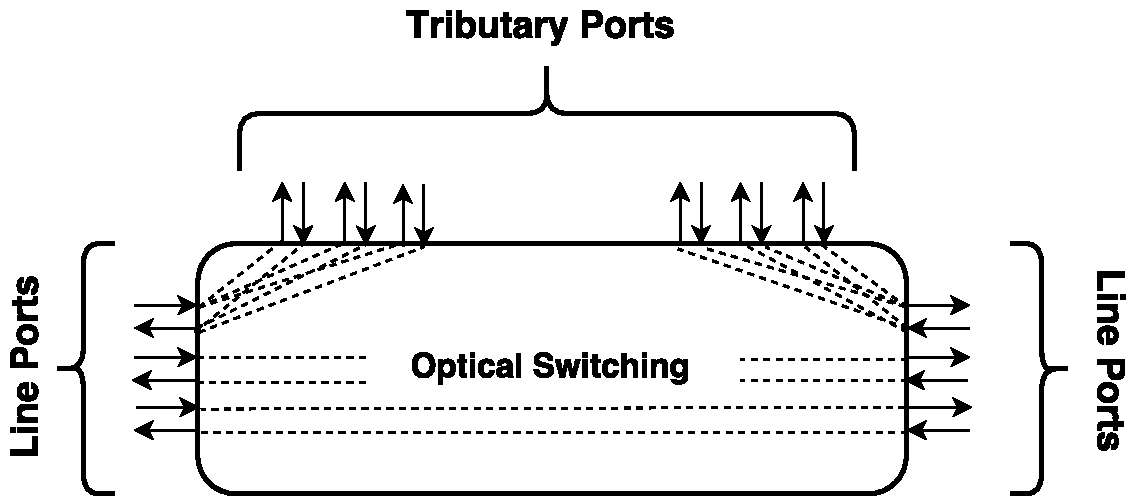
\includegraphics[width=8cm]{sdf/ILP/figures/oxc_design}
\caption{Design of a optical switching.}
\label{oxc_design}
\end{figure}

Through the previous image, we can conclude in a simple way that the optical cost is the sum of the fixed cost of the optical connection with the total cost of all the optical ports.
Therefore the optical cost in monetary units (e.g. euros, or dollars), $C_{OXC}$, is given by equation \ref{Capex_Node_OXC}

\begin{equation}
C_{OXC} = \sum_{n=1}^{N} N_{oxc,n} \bigg( \gamma_{o0} + \gamma_{o1} P_{oxc,n} \bigg)
\label{Capex_Node_OXC}
\end{equation}

\noindent
where
\begin{itemize}
\item{$N$				$\rightarrow$	Total number of nodes, N $\in \mathbb{N}$}
\item{$N_{oxc,n}$		$\rightarrow$	Binary variable indicating if node $n$ is used, $N_{oxc,n} \in {0, 1}$}
\item{$\gamma_{o0}$ 	$\rightarrow$	OXC cost in monetary units (e.g. euros, or dollars)}
\item{$\gamma_{o1}$ 	$\rightarrow$	OXC port cost in monetary units (e.g. euros, or dollars) }
\item{$P_{oxc,n}$	    $\rightarrow$	Number of ports of the optical switch}
\end{itemize}


\vspace{10pt}
We have to take into account that the calculated value for the variable $P_{exc,c,n}$ and $P_{oxc,n}$ will depend on the mode of transport used (opaque, transparent or translucent) but in next subsections will be explained how these values are calculated for each specific transport mode.\\

All transport modes require the routing of the demands. In this work we assume that the routing is performed by the ILP model instead of feeding it with candidate paths.\\
The flow conservation constraints ensures that, for each $(o,d)$ pair we route Z units of flow from node $o$ to node $d$. The flow conservation constraints are as follows \cite{teserui}:

\begin{equation}
\sum_{j=1\textbackslash \{o\}}^{N} f_{ij}^{od} = Z  \qquad \qquad \qquad \qquad \qquad \qquad \qquad \qquad \qquad
\forall(o,d) : o < d, \forall i: i = o
\label{ILPOpaque1_CAPEX}
\end{equation}
\noindent
Constraint \ref{ILPOpaque1_CAPEX} states that for each $(o,d)$ pair the node $o$ (being the source of the flow) sends Z units through one or more links $(i,j)$ such as $o=i$. The variable Z depends of the transport mode and survivability mechanism.

\begin{equation}
\sum_{j=1\textbackslash \{o\}}^{N} f_{ij}^{od} = \sum_{j=1\textbackslash \{d\}}^{N} f_{ji}^{od}   \qquad \qquad \qquad \qquad \qquad \qquad \qquad \qquad
\forall(o,d) : o < d, \forall i: i \neq o,d
\label{ILPOpaque2_CAPEX}
\end{equation}
\noindent
Constraint \ref{ILPOpaque2_CAPEX} ensures that the remaining nodes, being neither origin or destination of the flow, the amount of received flow have to be send.

\begin{equation}
\sum_{j=1\textbackslash \{d\}}^{N} f_{ji}^{od} = Z  \qquad \qquad \qquad \qquad \qquad \qquad \qquad \qquad \qquad \qquad
\forall(o,d) : o < d, \forall i: i = d
\label{ILPOpaque3_CAPEX}
\end{equation}
\noindent
Constraint \ref{ILPOpaque3_CAPEX} states that the destination node, $d$, has to receive those Z units of flow.\\

Finally, one aspect to be taken into account is the cost of the equipment used in the network. Through the table \ref{table_cost_ilp} we can see the cost in euros of the equipment.

\begin{table}[h!]
\centering
\begin{tabular}{|| c | c | c||}
 \hline
 Equipment & Symbol & Cost \\
 \hline\hline
 OLT without transponders & $\gamma_0^{OLT}$ & 15 000 \euro \\
 Transponder & $\gamma_1^{OLT}$ & 5 000 \euro/Gb \\
 Unidirectional Optical Amplifier & $c^R$ & 4 000 \euro \\
 EXC & $\gamma_{e0}$ & 10 000 \euro \\
 OXC & $\gamma_{o0}$ & 20 000 \euro \\
 EXC Port for line ports & $\gamma_{e1,-1}$ & 100 000 \euro /port\\
 EXC Port for ODU0 & $\gamma_{e1,0}$ & 10 \euro /port\\
 EXC Port for ODU1 & $\gamma_{e1,1}$ & 15 \euro /port\\
 EXC Port for ODU2 & $\gamma_{e1,2}$ & 30 \euro /port\\
 EXC Port for ODU3 & $\gamma_{e1,3}$ & 60 \euro /port\\
 EXC Port for ODU4 & $\gamma_{e1,4}$ & 100 \euro /port\\
 OXC Port & $\gamma_{o1}$ & 2 500 \euro /port \\
 \hline
\end{tabular}
\caption{Table of costs used to calculate CAPEX using ILP models \cite{aulas}.}
\label{table_cost_ilp}
\end{table}


%Subsection with the different transport mode
\clearpage

\subsection{Opaque transport mode}\label{ILP_Opaque_Mode}

Before carrying out the description of the objective function we must take into account the following particularity of this mode of transport:
\begin{itemize}
  \item $N_{OXC,n}$ = 0, \quad $\forall$ n
  \item $N_{EXC,n}$ = 1, \quad $\forall$ n that process traffic
\end{itemize}

\vspace{11pt}
The objective function of following the ILP is a minimization of the CAPEX through the equation \ref{Capex} where in this case for the cost of nodes we only have in consideration the electric cost \ref{Capex_Node_EXC} because of the particularity previously mentioned.
In this case the value of $P_{exc,c,n}$ is obtained by equation \ref{EXC_pexc1_opaque} for long-reach and by the equation \ref{EXC_pexc2_opaque} for short-reach.\\

As previously mentioned, equation \ref{EXC_pexc1_opaque} refers to the number of long-reach ports of the electrical switch with bit-rate -1 in node n, $P_{exc,-1,n}$, i.e. the number of line ports of node n which can be calculated as

\begin{equation}
P_{exc,-1,n} = \sum_{j=1}^{N} w_{nj}
\label{EXC_pexc1_opaque}
\end{equation}
\vspace{11pt}

\noindent
where $w_{nj}$ is the number of optical channels between node $n$ and node $j$.\\

As previously mentioned, equation \ref{EXC_pexc2_opaque} refers to the number of short-reach ports of the electrical switch with bit-rate c in node n, $P_{exc,c,n}$, i.e. the number of tributary ports with bit-rate c in node n which can be calculated as

\begin{equation}
P_{exc,c,n} = \sum_{d=1}^{N} D_{nd,c}
\label{EXC_pexc2_opaque}
\end{equation}

\vspace{11pt}
\noindent
where $D_{nd,c}$ are the client demands between nodes $n$ and $d$ with bit rate $c$.\\

In this case there is the following particularity:

\begin{itemize}
  \item When $n$=$d$ the value of client demands is always zero, i.e, $D_{nn,c}=0$
\end{itemize}


\subsection{Transparent transport mode}\label{ILP_Transp_Mode}

Once again in this case it is necessary to minimize CAPEX through equation \ref{Capex} where in this case for the cost of nodes we have in consideration electric \ref{Capex_Node_EXC} and optical cost \ref{Capex_Node_OXC}. In this case the value of $P_{exc,c,n}$ is obtained by equation \ref{EXC_pexc1_transparent} for short-reach and by the equation \ref{EXC_pexc2_transparent} for long-reach and the value of $P_{oxc,n}$ is obtained by equation \ref{OXC_poxc_transparent}.\\

The equation \ref{EXC_pexc1_transparent} refers to the number of short-reach ports of the electrical switch with bit-rate $c$ in node $n$, $P_{exc,c,n}$, i.e. the number of tributary ports with bit-rate $c$ in node $n$ which can be calculated as

\begin{equation}
P_{exc,c,n} = \sum_{d=1}^{N} D_{nd,c}
\label{EXC_pexc1_transparent}
\end{equation}

\noindent
where $D_{nd,c}$ are the client demands between nodes $n$ and $d$ with bit rate $c$.\\

In this case there is the following particularity:
\begin{itemize}
  \item When $n$=$d$ the value of client demands is always zero, i.e, $D_{nn,c}=0$
\end{itemize}

As previously mentioned, the equation \ref{EXC_pexc2_transparent} refers to the number of long-reach ports of the electrical switch with bit-rate -1 in node n, $P_{exc,-1,n}$, i.e. the number of add ports of node n which can be calculated as

\begin{equation}
P_{exc,-1,n} = \sum_{j=1}^{N} \lambda_{nj}
\label{EXC_pexc2_transparent}
\end{equation}

\noindent
where $\lambda_{nj}$ is the number of optical channels between node $n$ and node $j$.\\

The equation \ref{OXC_poxc_transparent} refers to the number of ports in optical switch in node n, $P_{oxc,n}$, i.e. the number of line ports and the number of adding ports of node n which can be calculated as

\begin{equation}
P_{oxc,n} = \sum_{j=1}^{N} f_{nj}^{od} + \sum_{j=1}^{N} \lambda_{nj}
\label{OXC_poxc_transparent}
\end{equation}

\noindent
where $f_{nj}^{od}$ refers to the number of line ports for all demand pairs (od) and $\lambda_{nj}$ refers to the number of add ports.\\

In this case, again, the specific variables depend on the mode of survivability. With this in mind in the next chapter we can calculate CAPEX.\\


\subsection{Translucent transport mode}\label{ILP_Transluc_Mode}

The translucent mode has the particularity of while some nodes use electrical and optical part others use only electrical part. But for a better definition of the model we will take into account the following particularities:
\begin{itemize}
  \item $N_{OXC,n}$ = 1, \quad $\forall$ n that process traffic
  \item $N_{EXC,n}$ = 1, \quad $\forall$ n that process traffic
\end{itemize}

For this mode of transport it is also necessary to minimize CAPEX through equation \ref{Capex} where in this case for the cost of nodes we have in consideration electric \ref{Capex_Node_EXC} and optical cost \ref{Capex_Node_OXC}. In this case the value of $P_{exc,c,n}$ is obtained by equation \ref{EXC_pexc1_transluc} for short-reach and by the equation \ref{EXC_pexc2_transluc} for long-reach and the value of $P_{oxc,n}$ is obtained by equation \ref{OXC_poxc_transluc}.\\

The equation \ref{EXC_pexc1_transluc} refers to the number of short-reach ports of the electrical switch with bit-rate $c$ in node $n$, $P_{exc,c,n}$, i.e. the number of tributary ports with bit-rate $c$ in node $n$ which can be calculated as

\begin{equation}
P_{exc,c,n} = \sum_{d=1}^{N} D_{nd,c}
\label{EXC_pexc1_transluc}
\end{equation}

\noindent
where $D_{nd,c}$ are the client demands between nodes $n$ and $d$ with bit rate $c$.\\

In this case there is the following particularity:
\begin{itemize}
  \item When $n$=$d$ the value of client demands is always zero, i.e, $D_{nn,c}=0$
\end{itemize}

As previously mentioned, the equation \ref{EXC_pexc2_transluc} refers to the number of long-reach ports of the electrical switch with bit-rate -1 in node n, $P_{exc,-1,n}$, i.e. the number of add ports of node n which can be calculated as

\begin{equation}
P_{exc,-1,n} = \sum_{k=1}^{N} \lambda_{nk}
\label{EXC_pexc2_transluc}
\end{equation}

\noindent
where $\lambda_{nk}$ is the number of optical channels between lightpath $n$ and node $k$.\\

The equation \ref{OXC_poxc_transluc} refers to the number of ports in optical switch in node n, $P_{oxc,n}$, i.e. the number of line ports and the number of adding ports of node n which can be calculated as

\begin{equation}
P_{oxc,n} = \sum_{j=1}^{N} f_{nj}^{pk} + \sum_{k=1}^{N} \lambda_{nk}
\label{OXC_poxc_transluc}
\end{equation}

\noindent
where $f_{nj}^{pk}$ refers to the number of line ports for all lightpath pairs $(p,k)$ and $\lambda_{nk}$ refers to the number of add ports.\\

Taking into account that the variables defined previously for this mode of transport depend on the mode of survivability, in the following chapter it is already possible to calculate CAPEX.\\



%Section CAPEX analytical
\clearpage

\section{CAPEX}\label{analytical_CAPEX}
\begin{tcolorbox}	
\begin{tabular}{p{2.75cm} p{0.2cm} p{10.5cm}} 	
\textbf{Student Name}  &:& Tiago Esteves    (October 03, 2017 - )\\
\textbf{Goal}          &:& Implement of the analytical model to obtain the best possible CAPEX of a given network.
\end{tabular}
\end{tcolorbox}
\vspace{11pt}

The cost of a telecommunications network can be divided into CAPEX and OPEX.
CAPEX is the amount of money needed to set up and install a particular network.
OPEX is the amount of money needed to run this network as well as its maintenance and operation over time.
In this section we will only focus on CAPEX, that is, the costs of installing a particular network.
As we know the telecommunications networks are made up of links and nodes, so it is possible to define the CAPEX as being the sum of the cost of links and cost of nodes.
This can be said that the CAPEX cost in monetary units, $C_C$ is given by the equation \ref{analytical_Capex}

\begin{equation}
C_C = C_L + C_N
\label{analytical_Capex}
\end{equation}

\noindent
where $C_L$ is the Link cost and $C_N$ is the Node cost.\\

For this calculation first let's focus on the cost of the links. Where to calculate the cost of the Links, $C_L$, we will use the equation \ref{analytical_linkCosts}

\begin{equation}
C_L = \left(2 L \gamma_0^{OLT}\right) + \left(2 L \gamma_1^{OLT} \tau <w>\right) + \left(2 N^R c^R\right)
\label{analytical_linkCosts}
\end{equation}

\vspace{11pt}
\noindent
where
\begin{itemize}
\item{$\gamma_0^{OLT}$	$\rightarrow$	OLT cost in euros}
\item{$L$				$\rightarrow$	Number of bidirectional links}
\item{$\gamma_1^{OLT}$	$\rightarrow$	Transponder cost in euros}
\item{$<w>$             $\rightarrow$   Average number of optical channels}
\item{$\tau$		    $\rightarrow$	Traffic per port}
\item{$N^R$				$\rightarrow$	Total number of optical amplifiers}
\item{$c^R$				$\rightarrow$	Unidirectional Optical amplifiers cost in euros}
\end{itemize}

\vspace{11pt}
Looking at the equation \ref{analytical_linkCosts} we can see that we already have practically all the values of the variables used. Assuming that $\tau$ is 100 Gbits/s is thus only missing the number of optical amplifiers and the number of optical channels where they can be calculated by equation \ref{amplifiers} and \ref{optical_channels} respectively.

\begin{equation}
N^R = \sum\limits_{l=1}^L\left(\left\lceil\frac{len_l}{span}\right\rceil-1\right)
\label{amplifiers}
\end{equation}


\begin{itemize}
\item{$N^R$			$\rightarrow$ Total number of regenerators/amplifiers}
\item{$len_l$		$\rightarrow$ Length of link l}
\item{$span$		$\rightarrow$ Distance between amplifiers (assuming 100 km)}	
\end{itemize}	


\begin{equation}
<w> = \left( \frac{\lceil D \times <h> \rceil}{L} \right) \times \left( 1 + <k>\right)
\label{optical_channels}
\end{equation}


\begin{itemize}
\item{$<w>$		$\rightarrow$ Average number of optical channels}
\item{$D$  		$\rightarrow$ Number of unidirectional demands}
\item{$L$		$\rightarrow$ Number of unidirectional Links}	
\item{$<k>$		$\rightarrow$ Survivability coefficient}
\end{itemize}	

where:
\begin{equation}
D = \left(\frac{1}{2}\right) \times \left( 1 + \xi \right) \times \left(\frac{T_1}{\tau}\right)
\label{demands}
\end{equation}


\begin{itemize}
\item{$D$  		$\rightarrow$ Number of unidirectional demands}
\item{$\xi$		$\rightarrow$ Grooming coefficient}
\item{$T_1$		$\rightarrow$ Total unidirectional traffic}	
\item{$\tau$	$\rightarrow$ Traffic per port}
\end{itemize}

\vspace{11pt}
The next step is to take into account the cost of the nodes, but for this we must first know how a node is constituted. The nodes have an electrical part and an optical part so we can conclude that the cost of the nodes is given by the sum of these two parts thus obtaining the equation \ref{analytical_Capex_Node}.

\begin{equation}
C_N = C_{EXC} + C_{OXC}
\label{analytical_Capex_Node}
\end{equation}

\vspace{11pt}
To know the electric cost of the nodes that is given by equation \ref{analytical_electricalCost}.

\begin{equation}
C_{exc} = N \times \left( \gamma_{e0} + \left( \gamma_{e1} \times \tau \times <P_{exc}> \right) \right)
\label{analytical_electricalCost}
\end{equation}


\begin{itemize}
\item{$C_{exc}$		$\rightarrow$	Electrical ports cost}
\item{$N$			$\rightarrow$	Number of nodes}
\item{$\gamma_{e0}$	$\rightarrow$	EXC cost in euros}
\item{$\gamma_{e1}$	$\rightarrow$	EXC port cost in euros}
\item{$\tau$		$\rightarrow$	Traffic per port}
\item{$<P_{exc}>$   $\rightarrow$   Average number of ports of the electrical switch}
\end{itemize}

\vspace{11pt}
In relation to the optical part to know the optical cost of the nodes that is given by equation \ref{analytical_opticalCost}.

\begin{equation}
C_{oxc} = N \times \left( \gamma_{o0} + \left( \gamma_{o1} \times <P_{oxc}> \right) \right)
\label{analytical_opticalCost}
\end{equation}


\begin{itemize}
\item{$C_{oxc}$		$\rightarrow$	Optical ports cost}
\item{$N$			$\rightarrow$	Number of nodes}
\item{$\gamma_{o0}$	$\rightarrow$	OXC cost in euros}
\item{$\gamma_{o1}$	$\rightarrow$	OXC port cost in euros}
\item{$<P_{oxc}>$   $\rightarrow$   Average number of ports of the optical switch}
\end{itemize}

\vspace{10pt}
We have to take into account that the calculated value for the variable $<P_{exc}>$ and $<P_{oxc}>$ will depend on the mode of transport used (opaque, transparent or translucent) but later on it will be explained how these values are calculated for each specific transport mode.
Finally, for this we will also have to take into account the cost of the equipment used that can be consulted in table \ref{table_cost_analytical}.\\

\begin{table}[h!]
\centering
\begin{tabular}{|| c | c||}
 \hline
 Equipment & Cost \\
 \hline\hline
 OLT without transponders & 15000 \euro \\
 Transponder & 5000 \euro/Gb \\
 Unidirectional Optical Amplifier & 4000 \euro \\
 EXC & 10000 \euro \\
 OXC & 20000 \euro \\
 EXC Port & 1000 \euro /Gb/s\\
 OXC Port & 2500 \euro /porto \\
 \hline
\end{tabular}
\caption{Table with costs}
\label{table_cost_analytical}
\end{table}


%Subsection with the different transport mode
\clearpage

\subsection{Opaque transport mode}\label{analytical_Opaque_Mode}

Before carrying out the detailed description we must take into account the following peculiarities of this mode of transport:
\begin{itemize}
  \item $C_{oxc}$ = 0
  \item $\xi$ = 1
  \item $<k>$ = 0 or $<k>$ = $<kp>$ (depending of survivability)
\end{itemize}

The first particularity exists because in this mode of transport there is no optical cost, in the case of the second we are assuming that the grooming coefficient has value 1 and finally in the last particularity we are assuming that the survivability coefficient is zero when it is without survivability or $<kp>$ when it is with 1+1 protection where

\begin{equation}
<kp> = \frac{<h'>}{<h>}
\label{coefficient_protec}
\end{equation}

\vspace{13pt}
Finally looking at the equation \ref{analytical_electricalCost} we can see that we already have practically all the values with the exception of two variables. The tributary ports, $P_{TRIB}$, can be calculated through the ODU's matrices referred to in section \ref{Reference_Network_Traffic} and the average number of ports the electrical switch,$<P_{exc}>$, that can be calculated as

\begin{equation}
<P_{exc}> = <d> <h> \left(1 + <k>\right)
\label{Pexc_opaque}
\end{equation}

\noindent
where $<d>$ is the average number of demands, $<h>$ is the average number of hops and $<k>$	is the survivability coefficient. The number of ports of the electrical switch, in this case, is equal to the number of line ports since we already know the number of tributary ports.\\
The variable $<d>$ is calculated through the equation \ref{average_demand}

\begin{equation}
<d> = \frac{D}{N}
\label{average_demand}
\end{equation}


\subsection{Transparent transport mode}\label{analytical_Transp_Mode}

Once more, we must take into account the particularities of this mode of transport before executing the equation of the variables:
\begin{itemize}
  \item $\xi$ = 1.25
  \item $<k>$ = 0 or $<k>$ = $<kp>$ (depending of survivability)
\end{itemize}

The first particularity exists because we are assuming that the grooming coefficient has value 1.25 and finally in the last particularity we are assuming that the survivability coefficient is zero because it is without survivability or $<kp>$ when it is with 1+1 protection \cite{aulas} where

\begin{equation}
<kp> = \frac{<h'>}{<h>}
\label{coefficient_protec2}
\end{equation}

\vspace{13pt}
Finally looking at the equation \ref{analytical_electricalCost} we can see that we already have practically all the values with the exception of three variables. The tributary ports, $P_{TRIB}$, can be calculated through the ODU's matrices referred to in section \ref{Reference_Network_Traffic}, the average number of ports the electrical switch,$<P_{exc}>$, that can be calculated as

\begin{equation}
<P_{exc}> = <d>
\label{Pexc_transp}
\end{equation}

\noindent
and the average number of ports the optical switch,$<P_{oxc}>$, can be calculated as

\begin{equation}
<P_{oxc}> = <d> [1 + \left(1 + <k>\right) <h>]
\label{Poxc_transp}
\end{equation}

\noindent
where $<d>$ is the average number of demands, $<k>$	is the survivability coefficient and $<h>$ is the average number of hops.\\
The number of ports of the electrical switch, in this case, is equal to the number of add ports since we already know the number of tributary ports. The number of ports of the optical switch, in this case, is equal to the sum of the line ports with the add ports \cite{aulas}.\\


%%%%%%%%%%%%%%%%%%%%%%%%%%%%%%%%%%%%%%%%%%%%%%%%%%%%%%%%%%%%%%%%%%%%%%%%%%%%%%%%%%%%%%%%%%%%%%%%%%%%%%%%%%%%%%%%%%%%%%%%%%%%%

% References
\phantomsection
\addcontentsline{toc}{section}{References}
%
\renewcommand{\bibname}{References}
%\bibliographystyle{IEEEtran}
%\bibliography{rmorais}
%
%
% Generated by IEEEtran.bst, version: 1.13 (2008/09/30)
\begin{thebibliography}{10}
\providecommand{\url}[1]{#1}
\csname url@samestyle\endcsname
\providecommand{\newblock}{\relax}
\providecommand{\bibinfo}[2]{#2}
\providecommand{\BIBentrySTDinterwordspacing}{\spaceskip=0pt\relax}
\providecommand{\BIBentryALTinterwordstretchfactor}{4}
\providecommand{\BIBentryALTinterwordspacing}{\spaceskip=\fontdimen2\font plus
\BIBentryALTinterwordstretchfactor\fontdimen3\font minus
  \fontdimen4\font\relax}
\providecommand{\BIBforeignlanguage}[2]{{%
\expandafter\ifx\csname l@#1\endcsname\relax
\typeout{** WARNING: IEEEtran.bst: No hyphenation pattern has been}%
\typeout{** loaded for the language `#1'. Using the pattern for}%
\typeout{** the default language instead.}%
\else
\language=\csname l@#1\endcsname
\fi
#2}}
\providecommand{\BIBdecl}{\relax}
\BIBdecl

\bibitem{capex}
\BIBentryALTinterwordspacing
Wikipedia ``CAPEX,'' [Online]. Available: \url{https://pt.wikipedia.org/wiki/CAPEX}
\BIBentrySTDinterwordspacing

\bibitem{opex}
\BIBentryALTinterwordspacing
Wikipedia ``OPEX,'' [Online]. Available: \url{https://pt.wikipedia.org/wiki/OPEX}
\BIBentrySTDinterwordspacing

\bibitem{aulas}
A.~N. Pinto, ``Design of Optical Transport Networks,'' \emph{Aulas de redes opticas 2016-2017.}

\bibitem{teserui}
R.~M.~D. Morais, ``Planning and Dimensioning of Multilayer Optical Transport Networks.'' PhD thesis, Universidade de Aveiro, 2015.

\bibitem{ramas2010}
R. Ramaswami, K. N.~Sivarajan, and G. H. Sasaki, \emph{Optical Networks: A Practical Perspective}, Morgan Kaufmann, 2010.

\end{thebibliography} 